\subsection{Grobkonzept 4} \label{subsec:grobkonzept3}
\begin{table}[H]
\footnotesize
\begin{tabular}{>{\HY\RaggedRight}p{3cm} >{\HY\RaggedRight}p{3.5cm} >{\HY\RaggedRight}p{6cm} >{\HY\RaggedRight}p{1.2cm}}
\hline
\textbf{Bestandteil}&\textbf{Typ}&\textbf{Funktion}&\textbf{Anz.}\\
\hline

\rowcolor{dgelb}
\multicolumn{4}{l}{\textbf{Stromerzeugung}}\\
Rohrkette&&Umwandlung potenzielle Energie zu Rotation&6\\
Zahnrad&&Umdehungszahl für Generator anpassen&6\\
Generator&AC&Umwandlung in elektrische Energie&6\\
Gleichrichter&AC/DC Wandler&Wechselstrom zu Gleichstrom&6\\
DC/DC Konverter&&Verhindern das Strom zurückfliessen kann&6\\
Wechselrichter&&Umwandlung DC in AC (230V)&1\\

\rowcolor{dpink}
\multicolumn{4}{l}{\textbf{Kontrollsystem}}\\
PC&&Anlagesteuerung&1\\
SPS&Beckhof&Analoge und Digitale Aus- und Eingänge&1\\

\rowcolor{dgruen}
\multicolumn{4}{l}{\textbf{Abwassertechnik}}\\
Ventile&Absperrklappe&Umleitung in Fallleitung für Wartungsarbeiten am Wasserlift&74\\
Fallleitung&&Für Wartungsarbeiten&1\\

\hline
\end{tabular}
\end{table}
Im Grobkonzepts 4 wird die potenzielle Energie des Abwassers mit der Wasserlifttechnik ausgenutzt. Das Abwasser fliesst in eine Schaufel und wird in der Schaufel im Rohr nach unten transportiert. Somit erhält der Lift eine Bewegung nach unten und entleert am tiefsten Punkt das Abwasser. Die Drehbewegung, welche die Rohrkette erzeugt ist eher langsam. Daher müss die Drehbewegung mit einem Zahnradsystem verschnellert werden, damit die Mindestdrehzahl des Generators erreicht wird. Muss das System gewartet werden, wird das Abwasser in eine normale Fallleitung, mithilfe von Ventilen, umgeleitet. Damit der Strom der Turbinen zusammengeführt werden kann. Muss der Wechselstrom zuerst in Gleichstrom umgewandelt werden. Dieser wird auf einen DC-DC Konverter gelegt damit kein Strom zurück in den Generator fliessen kann. Anschliessen wird der Gleichstrom mit einem Wechselrichter auf Netz-Spannung umgewandelt. Ein Kontrollsystem steuert die Anlage und überwacht die Energiegewinnung und schreitet bei Störungen ein.

\newpage
\begin{wrapfigure}{r}{0.5\textwidth}
  \begin{center}
    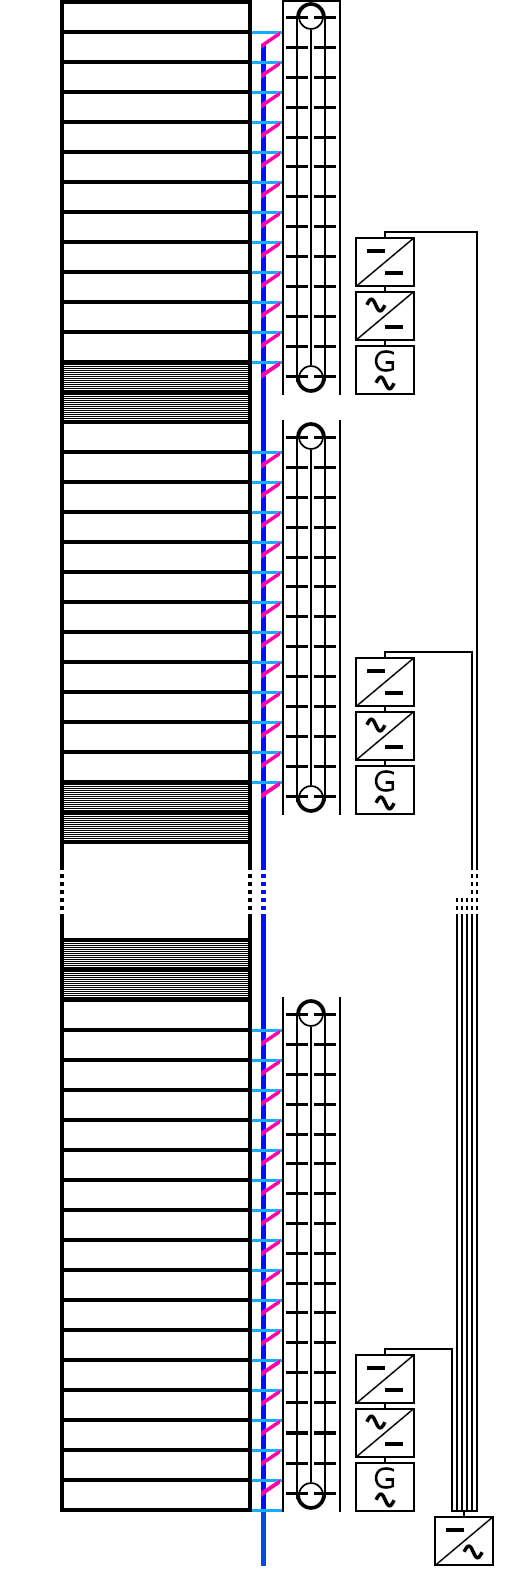
\includegraphics[width=0.48\textwidth]{grobkonzept4}
  \end{center}
  \caption{Grobkonzept 4}
\end{wrapfigure}
Die 5 oberen Lifte haben eine Länge von 66.08m, der unterste Lift 80.24m. Für Wartungsarbeiten existiert eine zusätzliche Leitung, die mittels Bypass angesteurt wird.

\textbf{Vorteile:}							\newline
+	kostengünstig							\newline
+ 	platzsparend								\newline
\newline
\textbf{Nachteile:}\newline
-	viele Ventile								\newline
-	Lufwtiderstand							\newline
-	ungeregelte Wasserflussmenge				\newline
\WFclear			
\newpage